\documentclass[11pt,a4paper]{article}

% --- Codificación, idioma y tipografía ---
\usepackage[utf8]{inputenc}
\usepackage[T1]{fontenc}
\usepackage[spanish,es-tabla]{babel}
\usepackage{lmodern}
\usepackage[margin=2.3cm]{geometry}

% --- Matemáticas, tablas y gráficos ---
\usepackage{amsmath,amssymb}
\usepackage{booktabs}
\usepackage{array}
\usepackage{multirow}
\usepackage{graphicx}
\usepackage{float}
\usepackage{xcolor}
\usepackage{tikz}
\usetikzlibrary{arrows.meta,positioning,shapes.geometric,fit,calc}

% --- Cajas visuales, listas y enlaces ---
\usepackage[most]{tcolorbox}
\usepackage{enumitem}
\usepackage{hyperref}

% --- Paleta corporativa verde bosque / azul marino ---
\definecolor{PrimaryGreen}{HTML}{0F5E4D}
\definecolor{SecondaryTeal}{HTML}{1D8A73}
\definecolor{NavyBlue}{HTML}{1E3A5F}
\definecolor{AccentCoral}{HTML}{E07A5F}
\definecolor{Slate}{HTML}{475569}
\definecolor{SoftBg}{HTML}{F4F8F7}
\definecolor{WarnBg}{HTML}{FFFBEB}
\definecolor{WarnBorder}{HTML}{D97706}

\hypersetup{
    colorlinks=true,
    linkcolor=PrimaryGreen,
    urlcolor=NavyBlue,
    citecolor=PrimaryGreen,
    pdftitle={Estimacion de carga termica de edificios con MLP - Grupo 02},
    pdfauthor={Grupo 02 - Sistemas Inteligentes y Machine Learning}
}

\newtcolorbox{cajasimple}[2][PrimaryGreen]{
    colback=SoftBg,
    colframe=#1,
    fonttitle=\bfseries,
    title=#2,
    boxrule=0.9pt,
    arc=3pt,
    left=8pt,
    right=8pt,
    top=6pt,
    bottom=6pt
}

\newtcolorbox{cajaalerta}[1]{
    colback=WarnBg,
    colframe=WarnBorder,
    fonttitle=\bfseries,
    title=#1,
    boxrule=0.9pt,
    arc=3pt,
    left=8pt,
    right=8pt,
    top=6pt,
    bottom=6pt
}

\begin{document}

% ==============================================================================
% PORTADA SENCILLA Y PROFESIONAL
% ==============================================================================
\begin{titlepage}
    \centering
    \vspace*{0.8cm}
    {\color{PrimaryGreen}\rule{\textwidth}{2pt}}\\[0.5cm]
    {\small\bfseries SISTEMAS INTELIGENTES Y MACHINE LEARNING \quad|\quad TRABAJO APLICATIVO — GRUPO 02}\\[1.1cm]
    {\Huge\bfseries\color{NavyBlue} Estimación de Carga Térmica de Edificios mediante una Red Neuronal Multicapa (MLP)}\\[0.5cm]
    {\Large\color{PrimaryGreen} Documentación completa del desarrollo en términos simples,\\ protocolo de 16 etapas y guion para diapositivas}\\[0.8cm]
    {\color{PrimaryGreen}\rule{\textwidth}{1pt}}\\[1.4cm]

    \begin{tcolorbox}[colback=SoftBg,colframe=PrimaryGreen,width=0.9\textwidth,arc=4pt]
        \textbf{Resumen ejecutivo del proyecto:}
        \begin{itemize}[leftmargin=1.2em,itemsep=3pt]
            \item \textbf{Objetivo:} Predecir cuánta energía de calefacción (\texttt{Y1}, en $\text{kWh/m}^2$) necesitará un edificio a partir de 8 características de diseño (\texttt{X1}–\texttt{X8}).
            \item \textbf{Datos:} 768 edificios simulados en \textit{Ecotect} (UCI Energy Efficiency, ID 242), almacenados localmente en el repositorio (\texttt{data/ENB2012\_data.xlsx}).
            \item \textbf{Modelo MLP ganador:} Arquitectura \textbf{MLP (32, 16) con ReLU} (1,089 parámetros entrenables).
            \item \textbf{Desempeño en Test (116 edificios nunca vistos):} $\text{RMSE} = \mathbf{0.4970\text{ kWh/m}^2}$, $\text{MAE} = \mathbf{0.3757\text{ kWh/m}^2}$ y $R^2 = \mathbf{0.9974}$. Reduce el error en más de \textbf{5 veces} frente a la Regresión Lineal ($\text{RMSE} = 2.7612$) y compite a la par con Random Forest ($\text{RMSE} = 0.5406$).
            \item \textbf{Repositorio autocontenido:} Incluye datos, modelos entrenados, figuras, notebook ejecutado y dashboard moderno en Streamlit (\texttt{app.py}).
        \end{itemize}
    \end{tcolorbox}

    \vfill
    \begin{tabular}{rl}
        \textbf{Asignatura:} & Sistemas Inteligentes y Machine Learning \\
        \textbf{Grupo:} & Grupo 02 — Perceptrón Multicapa (MLP) \\
        \textbf{Herramientas:} & Python 3.13, Scikit-learn 1.9.1, Pandas, Plotly y Streamlit \\
        \textbf{Semilla reproducible:} & \texttt{SEED = 42} \\
        \textbf{Integrantes:} & \underline{\hspace{6.8cm}} \\
        \textbf{Fecha:} & \underline{\hspace{6.8cm}}
    \end{tabular}
    \vspace*{0.8cm}
\end{titlepage}

\tableofcontents
\newpage

% ==============================================================================
% SECCIÓN 1: EXPLICACIÓN SIMPLE DEL PROBLEMA Y LOS DATOS
% ==============================================================================
\section{¿De qué trata el proyecto? (Explicación en palabras simples)}

Imagina que trabajamos en una \textbf{consultora de eficiencia energética}. Un arquitecto está diseñando un edificio nuevo y necesita saber cuánta energía va a consumir en calefacción durante el año (\textbf{variable objetivo $Y_1$}, medida en $\text{kWh/m}^2$) antes de construirlo.

Hacer una simulación física completa en un programa de ingeniería térmica toma tiempo cada vez que el arquitecto cambia una ventana o gira el edificio. Por eso, entrenamos una \textbf{Red Neuronal Multicapa (MLP)} que aprende directamente de 768 edificios ya simulados: tú le das 8 características del plano del edificio y la red responde al instante cuánta calefacción va a necesitar.

\subsection{¿Qué datos entran y qué sale? (Las variables $X_1$--$X_8$ y $Y_1$)}
Todos los datos provienen del repositorio oficial \textbf{UCI Machine Learning Repository — Energy Efficiency (ID 242)}, publicados por Tsanas y Xifara (2012) mediante simulaciones físicas en el programa \textit{Autodesk Ecotect}. El archivo oficial \texttt{ENB2012\_data.xlsx} tiene exactamente \textbf{768 filas} y \textbf{10 columnas}, sin ningún valor faltante ni filas duplicadas.

\begin{table}[H]
\centering
\caption{Diccionario simple de variables del dataset UCI Energy Efficiency (768 edificios).}
\label{tab:variables}
\small
\begin{tabular}{clllp{5.8cm}}
\toprule
\textbf{Código} & \textbf{Nombre} & \textbf{Tipo} & \textbf{Rango / Valores} & \textbf{Qué significa en palabras simples} \\
\midrule
\texttt{X1} & Compacidad relativa & Continua & $0.62 \text{ -- } 0.98$ & Qué tan compacto (cercano a un cubo) es el edificio. \\
\texttt{X2} & Área superficial & Continua & $514.5 \text{ -- } 808.5\text{ m}^2$ & Área total exterior (paredes + techo + suelo). \\
\texttt{X3} & Área de paredes & Continua & $245.0 \text{ -- } 416.5\text{ m}^2$ & Superficie total de las paredes verticales. \\
\texttt{X4} & Área de techo & Continua & $110.25 \text{ -- } 220.5\text{ m}^2$ & Superficie de la cubierta superior. \\
\texttt{X5} & Altura total & Continua & $3.5\text{ m}$ ó $7.0\text{ m}$ & 1 piso ($3.5\text{ m}$) o 2 pisos ($7.0\text{ m}$). \\
\texttt{X6} & Orientación & \textbf{Nominal} & $2, 3, 4, 5$ & Hacia dónde mira: 2=Norte, 3=Este, 4=Sur, 5=Oeste. \\
\texttt{X7} & Área acristalada & Continua & $0.0, 0.1, 0.25, 0.4$ & Porcentaje de ventanas respecto al piso (0\% a 40\%). \\
\texttt{X8} & Distribución ventanas & \textbf{Nominal} & $0, 1, 2, 3, 4, 5$ & Cómo se reparten: 0=Sin, 1=Uniforme, 2=N, 3=E, 4=S, 5=O. \\
\midrule
\texttt{Y1} & \textbf{Carga de calefacción} & \textbf{Meta ($y$)} & $6.01 \text{ -- } 43.10\text{ kWh/m}^2$ & \textbf{Lo que queremos predecir.} \\
\texttt{Y2} & Carga de refrigeración & Excluida & $10.90 \text{ -- } 48.03\text{ kWh/m}^2$ & Energía de aire acondicionado. \textbf{Prohibido usarla en $X$.} \\
\bottomrule
\end{tabular}
\end{table}

\begin{cajaalerta}{Regla de oro: ¿Por qué está prohibido usar $Y_2$ para predecir $Y_1$?}
En el archivo Excel aparecen dos salidas: calefacción ($Y_1$) y refrigeración ($Y_2$). Ambas están fuertemente correlacionadas ($r = \mathbf{0.9752}$). Si metiéramos $Y_2$ como dato de entrada estaríamos haciendo \textbf{trampa o fuga de datos (\textit{data leakage})}, porque en la vida real cuando un arquitecto diseña un plano nuevo \textbf{tampoco conoce $Y_2$}. En nuestro experimento de control, incluir $Y_2$ haría que una simple Regresión Lineal aparentara tener $\text{RMSE} = 1.3793$ ($R^2 = 0.9812$), un resultado totalmente engañoso e inutilizable en producción.
\end{cajaalerta}

% ==============================================================================
% SECCIÓN 2: TEORÍA EN TÉRMINOS SIMPLES + DIAGRAMA ORIGINAL
% ==============================================================================
\section{¿Cómo funciona un Perceptrón Multicapa (MLP) sin enredos?}

Una \textbf{Regresión Lineal} intenta explicar la calefacción como una suma simple de pesos multiplicados por cada variable (una línea o plano recto). El problema es que en física térmica las variables \textbf{interactúan entre sí de forma curva o no lineal}: por ejemplo, tener 40\% de ventanas afecta mucho más a un edificio alto de $7.0\text{ m}$ que a uno pequeño de $3.5\text{ m}$.

Un \textbf{Perceptrón Multicapa (MLP)} resuelve esto organizando neuronas artificiales en capas:
\begin{enumerate}[leftmargin=1.5em,itemsep=4pt]
    \item \textbf{Lo que hace cada neurona ($z = Wx + b$):} Toma las entradas $x$, las multiplica por unos pesos $W$ (que dicen qué tan importante es cada entrada) y les suma un ajuste o sesgo $b$. Hasta aquí sigue siendo una recta.
    \item \textbf{La chispa no lineal ($\text{ReLU}(z) = \max(0, z)$):} Si $z$ es negativo, la neurona se apaga ($0$); si es positivo, lo deja pasar tal cual. Gracias a este ``interruptor'' sencillo, al juntar varias neuronas la red puede doblar el espacio y aprender curvas complejas.
    \item \textbf{La capa final (Salida lineal):} Como $Y_1$ es un número continuo (como $24.5\text{ kWh/m}^2$) y no una categoría ``sí/no'', la última neurona suma los aportes de la última capa oculta \textbf{sin activación ReLU} para poder entregar cualquier número real.
    \item \textbf{Cómo aprende (Pérdida MSE + Retropropagación + Adam):}
    \begin{itemize}[leftmargin=1.2em]
        \item Al inicio los pesos $W$ son aleatorios y la red se equivoca bastante.
        \item Medimos qué tan lejos estuvo usando el \textbf{Error Cuadrático Medio (MSE)}: promedio de $(y_{\text{real}} - y_{\text{pred}})^2$.
        \item La \textbf{retropropagación (\textit{backpropagation})} calcula qué parte de la culpa del error tuvo cada peso desde la salida hacia atrás.
        \item El optimizador \textbf{Adam} ajusta los pesos poco a poco (controlado por la tasa de aprendizaje $\text{lr} = 0.005$) para bajar el error en cada vuelta o \textbf{época}.
    \end{itemize}
    \item \textbf{Cómo evitamos que ``memorice'' de más (Regularización L2 y Early Stopping):}
    \begin{itemize}[leftmargin=1.2em]
        \item \textbf{Regularización L2 ($\alpha$):} Penaliza que los pesos $W$ crezcan demasiado, obligando a la red a encontrar patrones suaves.
        \item \textbf{Early Stopping (Parada temprana):} Separa un pedacito interno del entrenamiento para vigilar el error y detiene el entrenamiento cuando la red deja de mejorar fuera de la muestra de ajuste.
    \end{itemize}
\end{enumerate}

\subsection{Diagrama original de la arquitectura MLP ganadora: \texttt{MLP (32, 16)}}
En la Figura~\ref{fig:arquitectura_mlp} se muestra el diagrama exigido para la sustentación, indicando dimensiones de tensores, activaciones, salida escalar y número exacto de parámetros entrenables.

\begin{figure}[H]
\centering
\begin{tikzpicture}[
    scale=0.92, transform shape,
    box/.style={draw, rounded corners=5pt, minimum width=2.8cm, minimum height=1.55cm, align=center, font=\small},
    arrow/.style={-{Stealth[length=2.8mm]}, thick, color=NavyBlue},
    backarrow/.style={-{Stealth[length=2.8mm]}, thick, dashed, color=AccentCoral}
]
    % Nodo 1: Entradas crudas
    \node[box, fill=SoftBg, draw=Slate] (raw) at (0,0) {
        \textbf{Entrada Cruda}\\
        $X \in \mathbb{R}^{N \times 8}$\\[2pt]
        \scriptsize 6 continuas + $X_6, X_8$
    };

    % Nodo 2: Preprocesamiento
    \node[box, fill=NavyBlue!8, draw=NavyBlue] (prep) at (3.6,0) {
        \textbf{Preprocesador}\\
        \scriptsize \texttt{StandardScaler} (6)\\
        \scriptsize \texttt{OneHotEncoder} ($4+6$)\\[2pt]
        \textbf{Tensor:} $\mathbb{R}^{N \times 16}$
    };

    % Nodo 3: Oculta 1
    \node[box, fill=PrimaryGreen!12, draw=PrimaryGreen] (h1) at (7.5,0) {
        \textbf{Capa Oculta 1}\\
        32 neuronas · \textbf{ReLU}\\
        $z_1 = W_1 x + b_1$\\
        $a_1 = \max(0, z_1)$\\[2pt]
        \scriptsize $W_1:(16,32)$, $b_1:(32,)$\\
        \textbf{\scriptsize 544 parámetros}
    };

    % Nodo 4: Oculta 2
    \node[box, fill=PrimaryGreen!12, draw=PrimaryGreen] (h2) at (11.3,0) {
        \textbf{Capa Oculta 2}\\
        16 neuronas · \textbf{ReLU}\\
        $z_2 = W_2 a_1 + b_2$\\
        $a_2 = \max(0, z_2)$\\[2pt]
        \scriptsize $W_2:(32,16)$, $b_2:(16,)$\\
        \textbf{\scriptsize 528 parámetros}
    };

    % Nodo 5: Salida
    \node[box, fill=AccentCoral!14, draw=AccentCoral] (out) at (14.9,0) {
        \textbf{Capa de Salida}\\
        1 neurona · \textbf{Lineal}\\
        $\hat{Y}_1 = W_3 a_2 + b_3$\\[2pt]
        \scriptsize $W_3:(16,1)$, $b_3:(1,)$\\
        \textbf{\scriptsize 17 parámetros}\\[2pt]
        \footnotesize $\hat{Y}_1 \in \mathbb{R}$ ($\text{kWh/m}^2$)
    };

    % Flechas forward
    \draw[arrow] (raw) -- (prep);
    \draw[arrow] (prep) -- (h1);
    \draw[arrow] (h1) -- (h2);
    \draw[arrow] (h2) -- (out);

    % Etiqueta Forward arriba
    \draw[-{Stealth[length=3mm]}, ultra thick, color=PrimaryGreen] (2.4,1.35) -- (15.0,1.35)
        node[midway, above, font=\small\bfseries, color=PrimaryGreen] {Flujo Forward (Inferencia): transformación capa a capa hasta $\hat{Y}_1$};

    % Flujo Backward abajo
    \node[draw=AccentCoral, fill=WarnBg, rounded corners=4pt, align=center, font=\footnotesize] (loss) at (9.4,-2.15) {
        \textbf{Pérdida MSE} $= \frac{1}{N}\sum (Y_1 - \hat{Y}_1)^2 + \alpha \|W\|_2^2$ \quad$\longrightarrow$\quad \textbf{Retropropagación + Adam} ($\text{lr}=0.005$)
    };
    \draw[backarrow] (out.south) |- (loss.east);
    \draw[backarrow] (loss.west) -| (h1.south);
    \draw[backarrow] (h2.south |- loss.north) -- (h2.south);

\end{tikzpicture}
\caption{Arquitectura feedforward del modelo ganador \texttt{MLP (32, 16), ReLU}: total de $544 + 528 + 17 = \mathbf{1{,}089}$ parámetros entrenables ($1{,}040$ pesos y $49$ sesgos).}
\label{fig:arquitectura_mlp}
\end{figure}

% ==============================================================================
% SECCIÓN 3: LAS 16 ETAPAS OBLIGATORIAS CON RESULTADOS REALES
% ==============================================================================
\section{Desarrollo de las 16 Etapas Metodológicas}

Todas las pruebas fueron ejecutadas de manera reproducible con semilla global \texttt{SEED = 42}, Python \texttt{3.13.5}, Scikit-learn \texttt{1.9.1} y Pandas \texttt{3.1.1}, cargando el dataset localmente desde \texttt{data/ENB2012\_data.xlsx} y \texttt{data/energy\_efficiency.csv}.

\begin{description}[leftmargin=0.8cm, style=nextline, itemsep=6pt]
    \item[Etapa 01 — Definición del problema:] Estimación rápida de carga térmica de calefacción para apoyar decisiones tempranas de diseño arquitectónico, dejando claro que los 768 registros provienen de simulaciones controladas en \textit{Ecotect} y no de mediciones reales con ocupación variable.
    \item[Etapa 02 — Tipo de aprendizaje:] Regresión supervisada tabular continua $f(X_1,\dots,X_8) \to Y_1$ medida en $\text{kWh/m}^2$.
    \item[Etapa 03 — Obtención y trazabilidad:] Dataset UCI Energy Efficiency (ID 242) guardado localmente en \texttt{data/ENB2012\_data.xlsx} y \texttt{data/energy\_efficiency.csv} ($768 \times 10$, 0 nulos, 0 duplicados).
    \item[Etapa 04 — Entradas, salidas y objetivo:] $X = \{X_1,\dots,X_8\}$, $y = Y_1$. Se excluye $Y_2$ de $X$ para evitar fuga de datos ($r = 0.9752$).
    \item[Etapa 05 — Análisis exploratorio (EDA):] Como muestran las Figuras~\ref{fig:eda_dist}, \ref{fig:eda_corr} y \ref{fig:eda_rel}, $Y_1$ tiene una clara distribución bimodal separada por la altura ($X_5$): edificios de 1 planta ($3.5\text{ m}$) rondan $6\text{--}20\text{ kWh/m}^2$ y los de 2 plantas ($7.0\text{ m}$) rondan $23\text{--}43\text{ kWh/m}^2$. Además, a mayor porcentaje acristalado ($X_7$), mayor demanda de calefacción por pérdidas térmicas en las ventanas.
\end{description}

\begin{figure}[H]
    \centering
    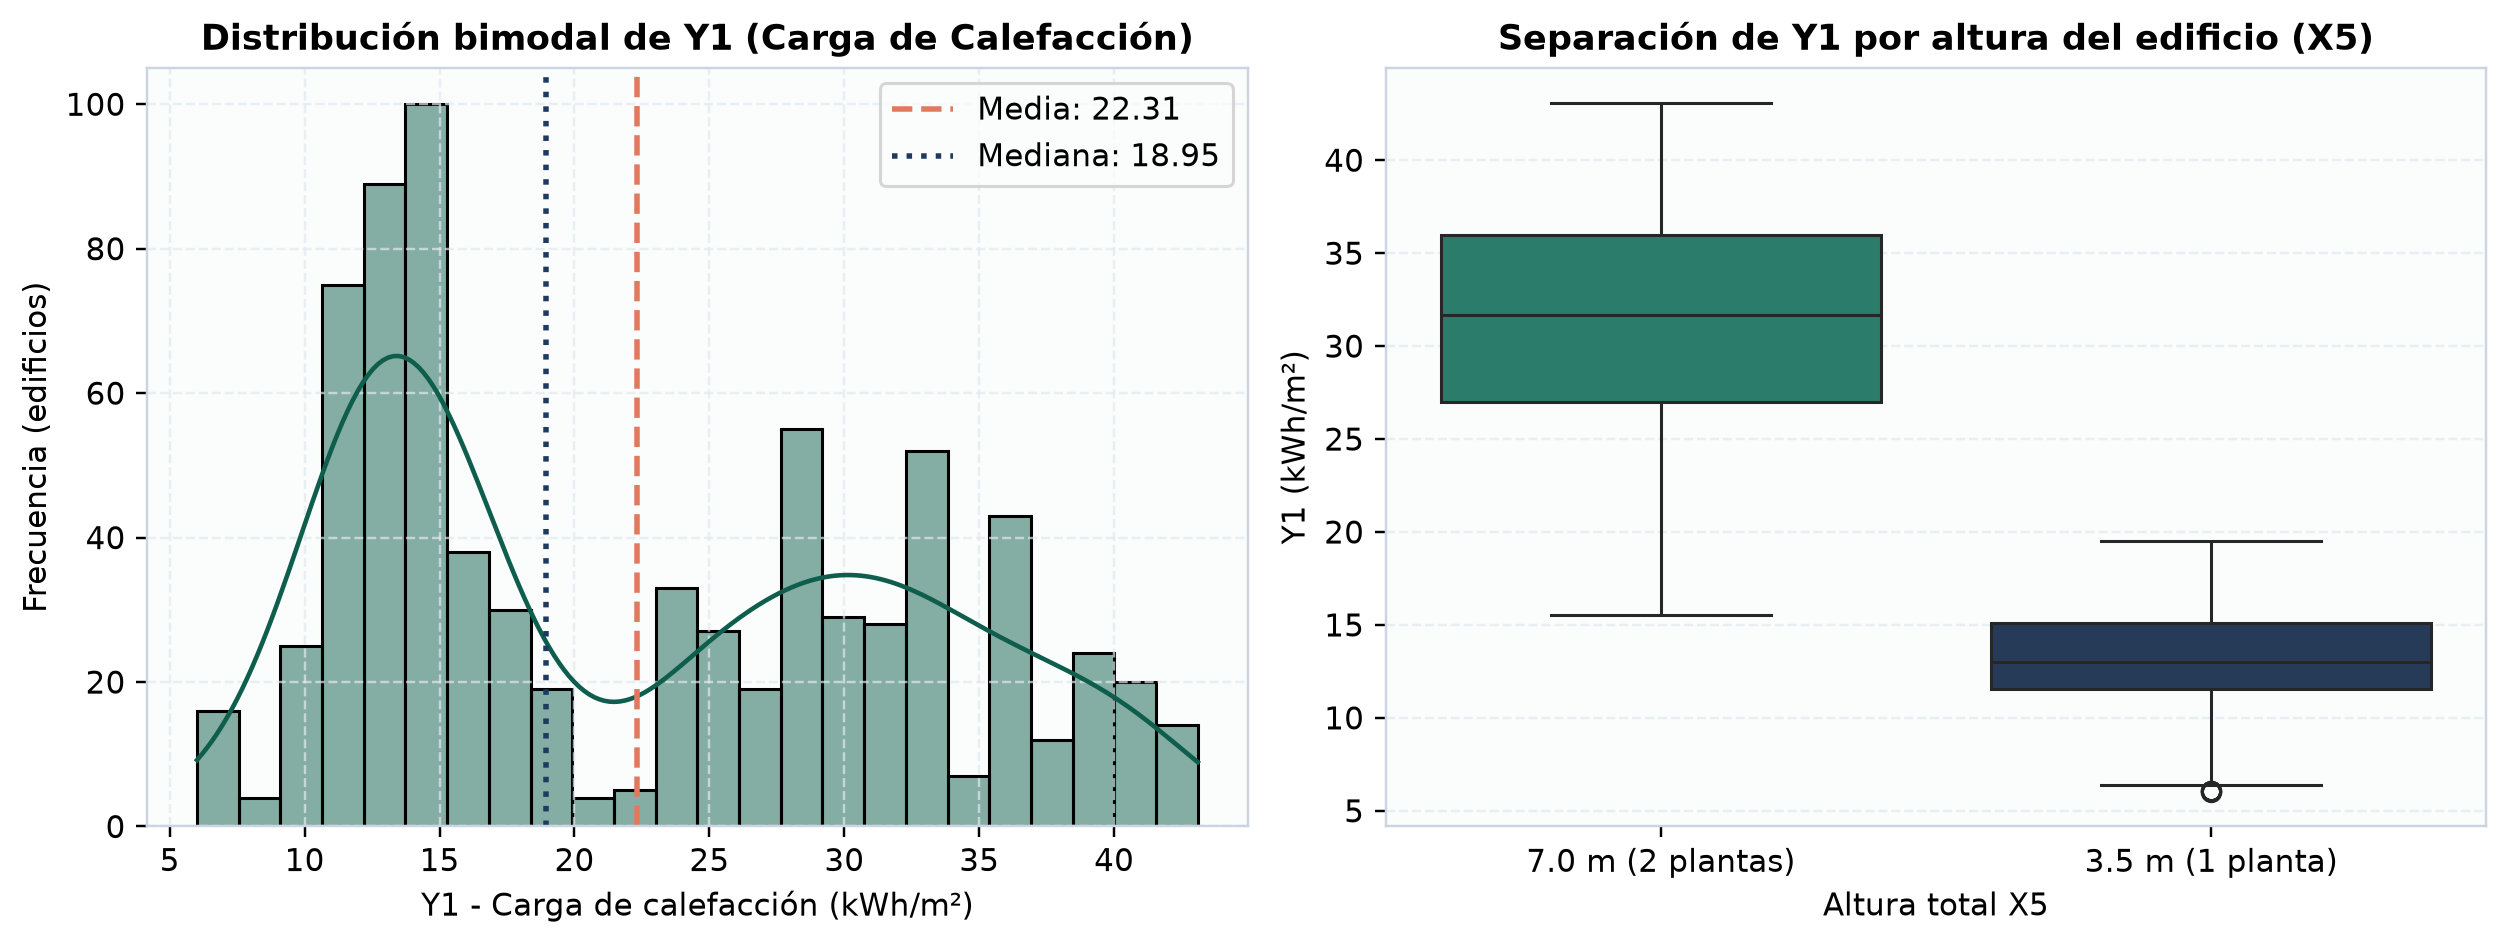
\includegraphics[width=0.95\textwidth]{../figures/fig01_distribucion_y1.png}
    \caption{Distribución bimodal de $Y_1$ (media $= 22.31$, mediana $= 18.95\text{ kWh/m}^2$) explicada por la altura del edificio $X_5$.}
    \label{fig:eda_dist}
\end{figure}

\begin{figure}[H]
    \centering
    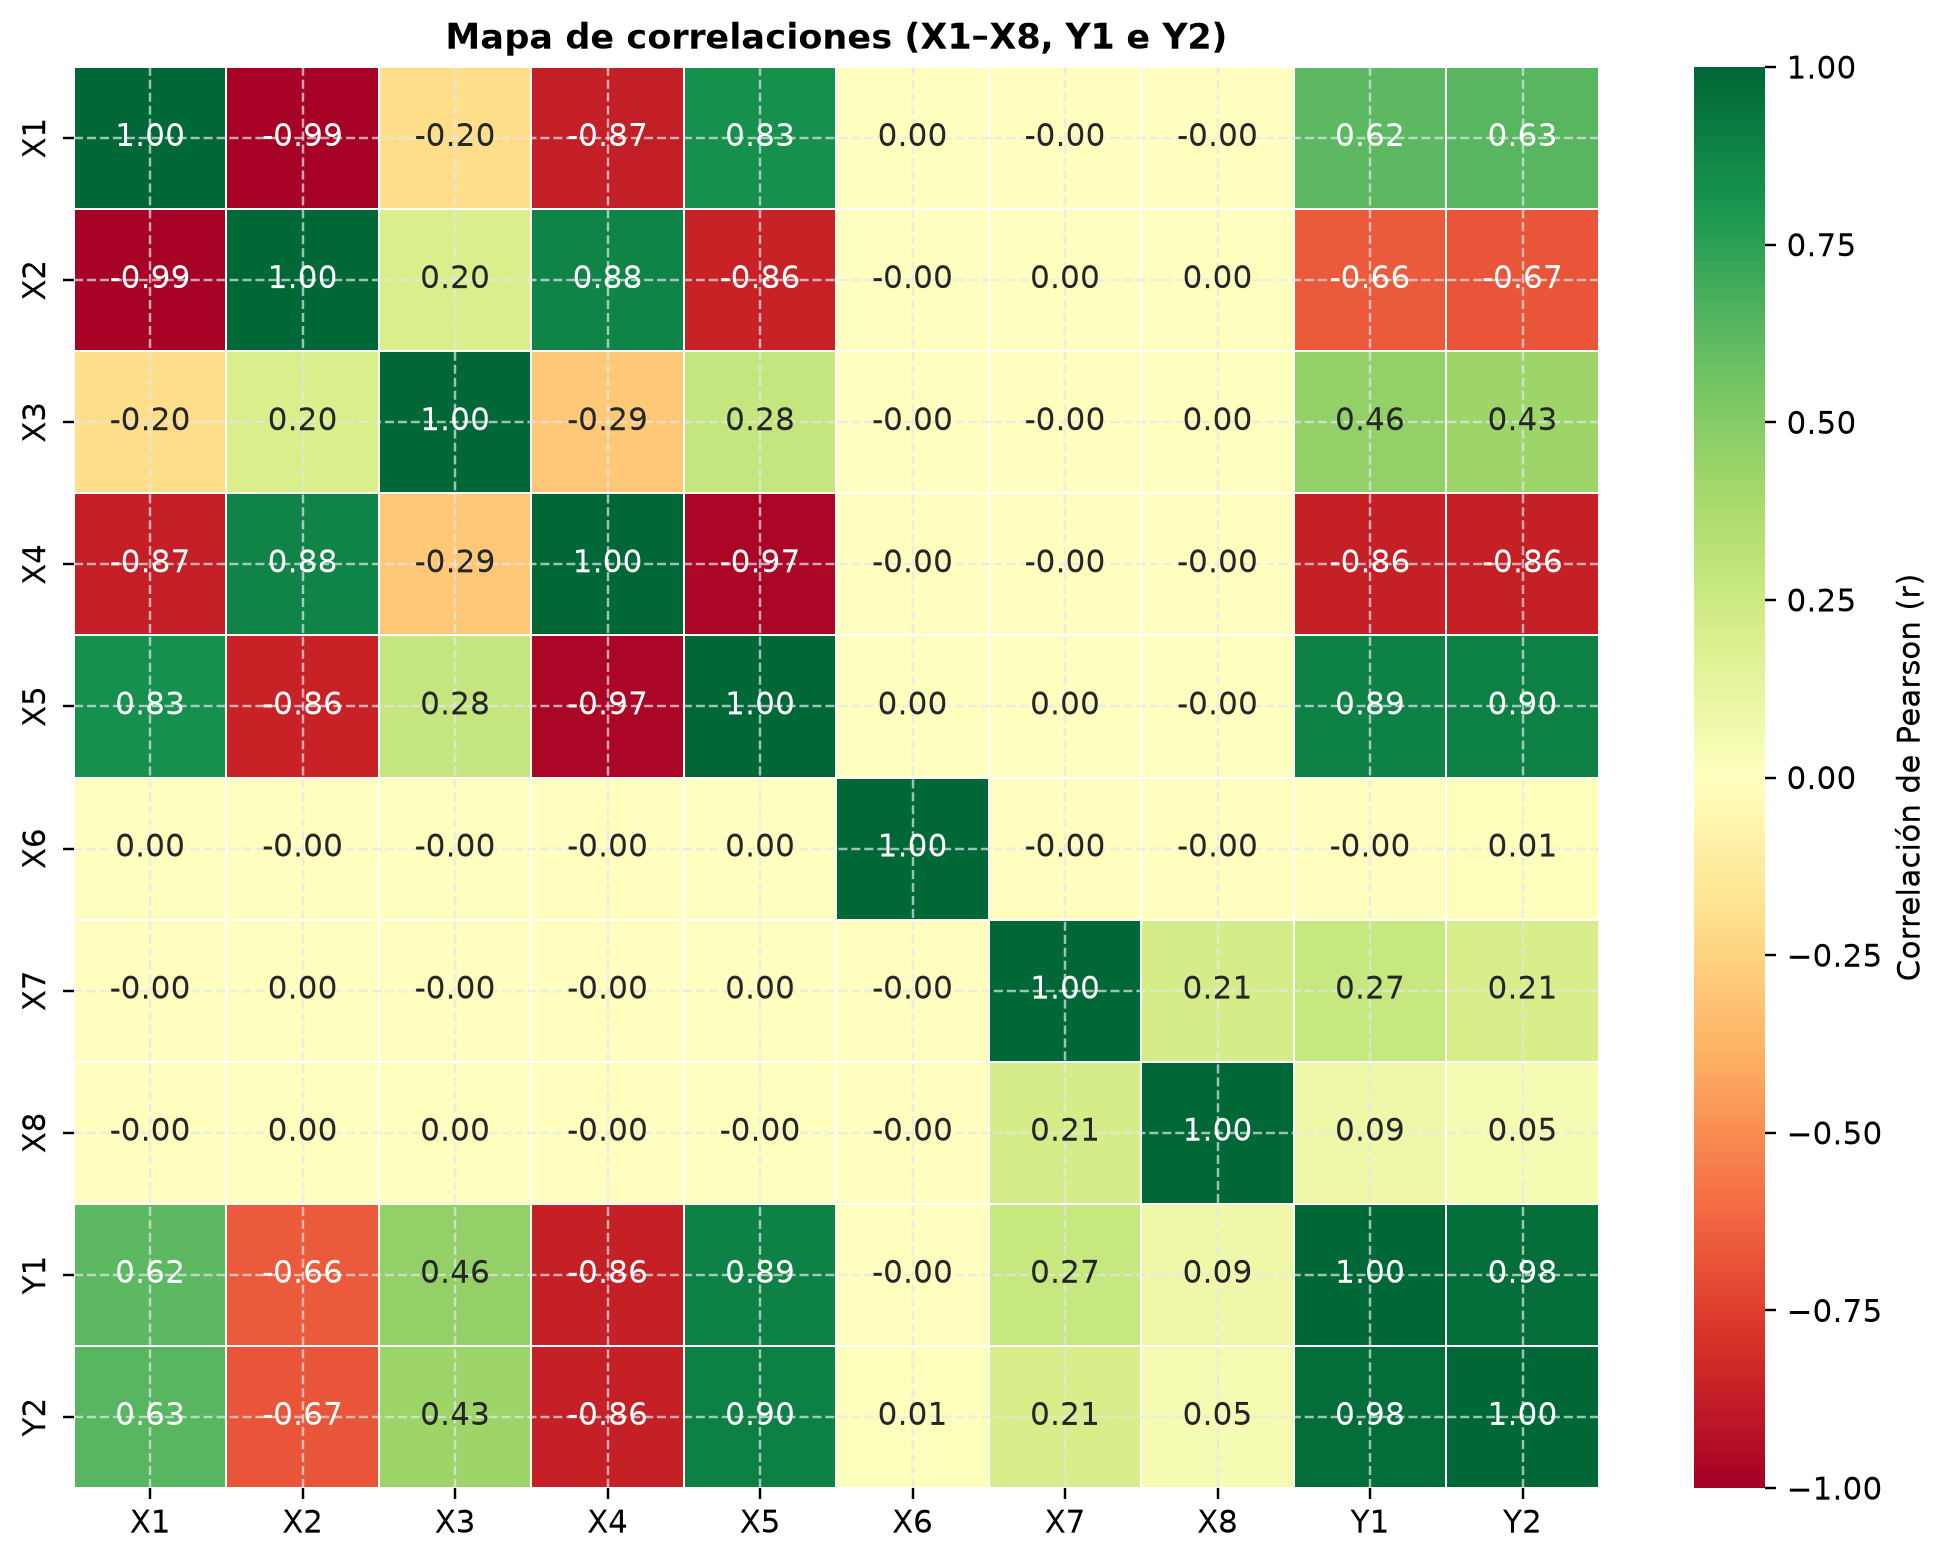
\includegraphics[width=0.78\textwidth]{../figures/fig02_correlaciones.png}
    \caption{Matriz de correlaciones de Pearson. Destaca la fuerte relación de $Y_1$ con $X_5$ ($+0.89$) y $X_4$ ($-0.86$), así como la aparente correlación casi nula con $X_6$ ($0.00$) por ser código nominal.}
    \label{fig:eda_corr}
\end{figure}

\begin{figure}[H]
    \centering
    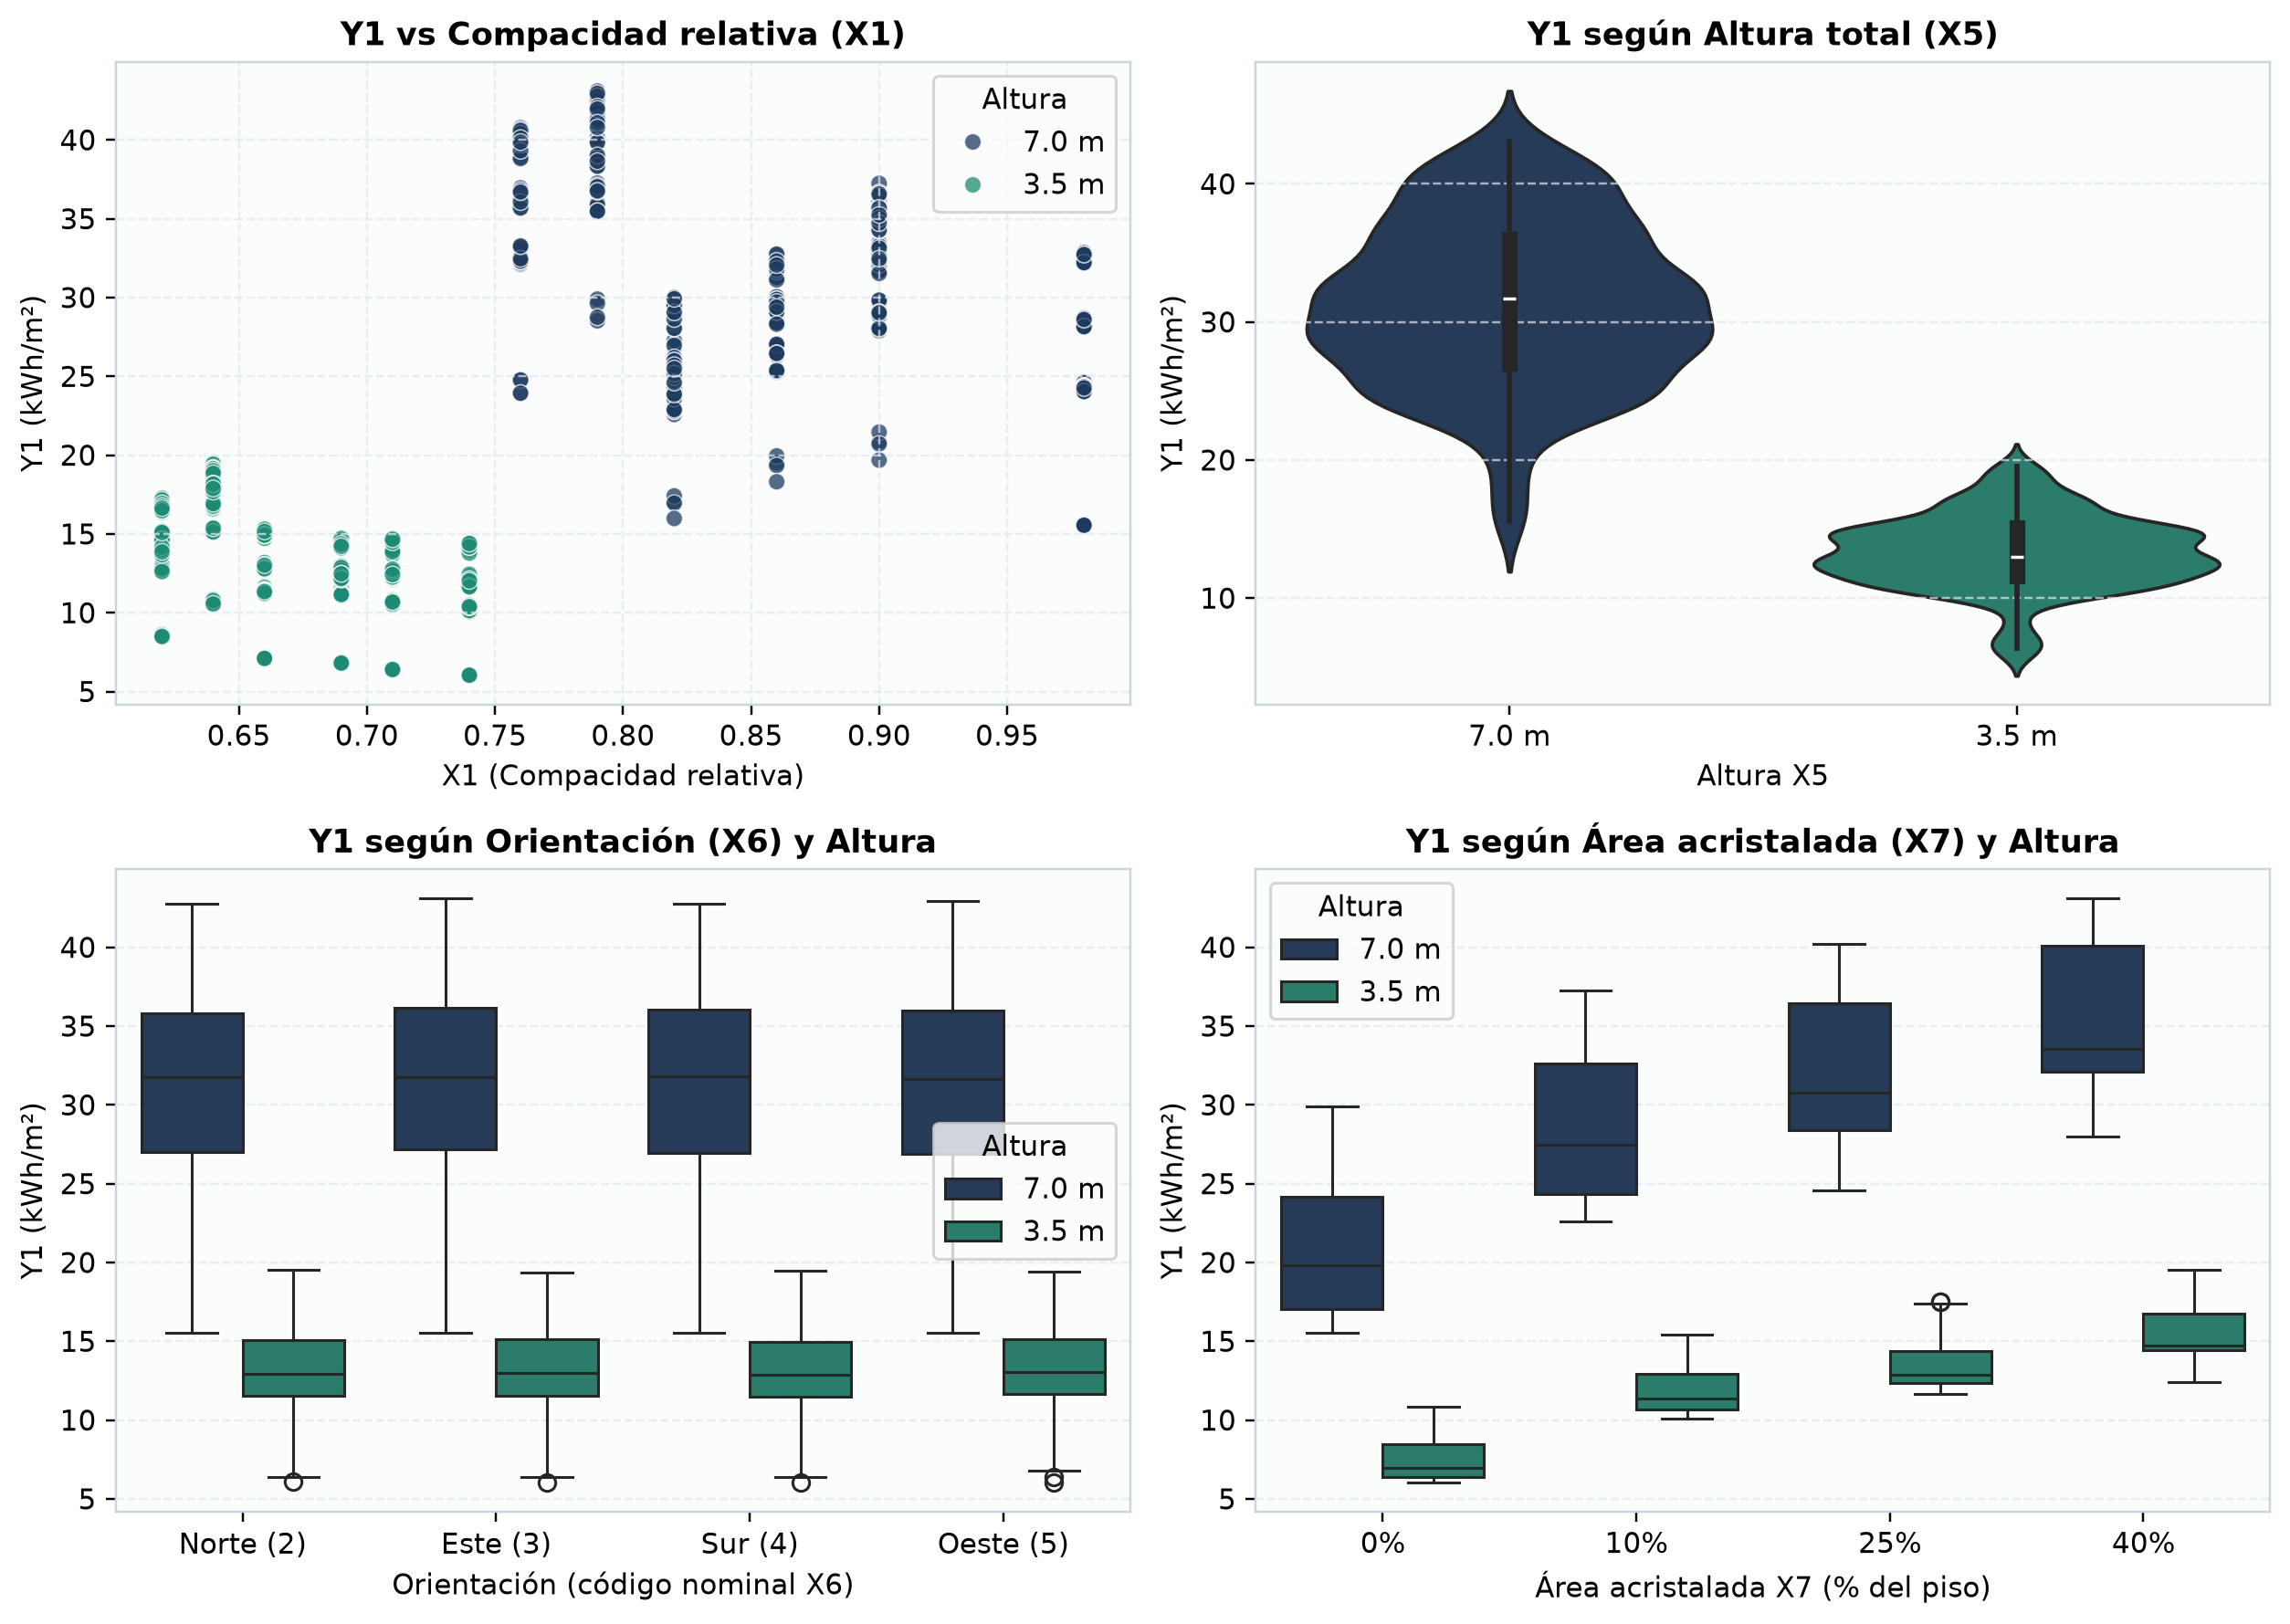
\includegraphics[width=0.95\textwidth]{../figures/fig03_eda_relaciones.png}
    \caption{Relación de $Y_1$ con compacidad ($X_1$), altura ($X_5$), orientación ($X_6$) y área acristalada ($X_7$).}
    \label{fig:eda_rel}
\end{figure}

\begin{description}[leftmargin=0.8cm, style=nextline, itemsep=6pt]
    \item[Etapa 06 — Separación experimental:] Partición estratificada por altura ($X_5$) y área acristalada ($X_7$) con \texttt{SEED = 42}: \textbf{Train = 537} (70\%), \textbf{Validation = 115} (15\%) y \textbf{Test = 116} (15\%). Las 12 formas arquitectónicas base ($X_1$--$X_5$) están presentes en los tres conjuntos, y el conjunto \textbf{Test permaneció completamente aislado} hasta la Etapa 15.
    \item[Etapa 07 — Preprocesamiento y efecto de \texttt{OneHotEncoder}:] Se imputan y estandarizan las 6 variables continuas con \texttt{StandardScaler} dentro de un \texttt{Pipeline} (ajustado solo en Train) y se aplica \texttt{OneHotEncoder} a $X_6$ (4 categorías) y $X_8$ (6 categorías), pasando de 8 a \textbf{16 dimensiones}. Como demuestra la Tabla~\ref{tab:onehot}, tratar $X_6$ y $X_8$ como códigos categóricos en lugar de números continuos redujo el RMSE de Validación del MLP de $0.7653$ a $\mathbf{0.4397\text{ kWh/m}^2}$ ($-42.5\%$).
\end{description}

\begin{table}[H]
\centering
\caption{Impacto real de codificar $X_6$ y $X_8$ con \texttt{OneHotEncoder} (métricas en Validación).}
\label{tab:onehot}
\small
\begin{tabular}{llcccc}
\toprule
\textbf{Modelo} & \textbf{Preprocesamiento} & \textbf{Cols.} & \textbf{Val MAE} & \textbf{Val RMSE} & \textbf{Val $R^2$} \\
\midrule
Regresión Lineal & Sin OneHot (numéricas crudas) & 8 & 2.0435 & 2.7518 & 0.9253 \\
Regresión Lineal & \textbf{Con OneHotEncoder ($X_6, X_8$)} & 16 & \textbf{1.9774} & \textbf{2.6172} & \textbf{0.9325} \\
\midrule
Random Forest (200) & Sin OneHot (numéricas crudas) & 8 & 0.3426 & 0.6395 & 0.9960 \\
Random Forest (200) & \textbf{Con OneHotEncoder ($X_6, X_8$)} & 16 & \textbf{0.3181} & \textbf{0.5701} & \textbf{0.9968} \\
\midrule
MLP (32, 16), ReLU & Sin OneHot (numéricas crudas) & 8 & 0.5163 & 0.7653 & 0.9942 \\
MLP (32, 16), ReLU & \textbf{Con OneHotEncoder ($X_6, X_8$)} & 16 & \textbf{0.3509} & \textbf{0.4397} & \textbf{0.9981} \\
\bottomrule
\end{tabular}
\end{table}

\begin{description}[leftmargin=0.8cm, style=nextline, itemsep=6pt]
    \item[Etapas 08 a 14 — Baselines, diseño MLP, experimentos A--D, curvas, CV y selección:]
    Evaluamos 3 baselines (\texttt{D0 DummyRegressor}, \texttt{D1 Regresión Lineal}, \texttt{D2 Random Forest}) y 5 configuraciones de MLP: \texttt{A} \texttt{(16)}, \texttt{B} \texttt{(32,16)}, \texttt{C1} \texttt{(64,32)} con mínima regularización ($\alpha = 10^{-6}$), \texttt{C2} \texttt{(64,32)} con L2 ($\alpha = 0.05$) y \texttt{C3} \texttt{(64,32)} con L2 + \textit{Early Stopping} ($\text{lr}=0.01$). Además ejecutamos \textbf{Validación Cruzada 5-Fold} sobre \texttt{Train+Val} ($n=652$) encapsulada en \texttt{Pipeline}.
\end{description}

\begin{table}[H]
\centering
\caption{Resultados reales de todos los experimentos en Validación, CV 5-Fold (Train+Val) y Test (SEED = 42).}
\label{tab:resultados}
\scriptsize
\begin{tabular}{clrrrrrrrrc}
\toprule
\textbf{Exp.} & \textbf{Modelo} & \textbf{Parám.} & \textbf{Ép.} & \textbf{T(s)} & \textbf{Train RMSE} & \textbf{Val RMSE} & \textbf{CV5 RMSE} & \textbf{Test MAE} & \textbf{Test RMSE} & \textbf{Test $R^2$} \\
\midrule
D0 & DummyRegressor (Media) & 1 & 1 & 0.034 & 10.1692 & 10.0731 & 10.1719 & 8.7625 & 9.6895 & -0.0003 \\
D1 & Regresión Lineal (OneHot) & 17 & 1 & 0.044 & 2.8251 & 2.6172 & 2.8357 & 1.9396 & 2.7612 & 0.9188 \\
D2 & Random Forest (200 árb.) & 133,398 & 1 & 0.736 & 0.2067 & 0.5701 & 0.5343 & 0.3632 & 0.5406 & 0.9969 \\
\midrule
A & MLP (16), ReLU & 289 & 2000 & 1.342 & 0.6551 & 0.8435 & 0.7752 & 0.5341 & 0.7480 & 0.9940 \\
\textbf{B} & \textbf{MLP (32, 16), ReLU} & \textbf{1,089} & \textbf{1909} & \textbf{2.736} & \textbf{0.2326} & \textbf{0.4404} & \textbf{0.5767} & \textbf{0.3757} & \textbf{0.4970} & \textbf{0.9974} \\
C1 & MLP (64, 32), $\alpha=10^{-6}$ & 3,201 & 1882 & 5.057 & 0.1139 & 0.5361 & 0.5610 & 0.4605 & 0.6248 & 0.9958 \\
C2 & MLP (64, 32), L2 $\alpha=0.05$ & 3,201 & 1008 & 2.057 & 0.2838 & 0.6205 & 0.6342 & 0.4151 & 0.5736 & 0.9965 \\
C3 & MLP (64, 32), L2 + EarlyStop & 3,201 & 533 & 1.431 & 0.2812 & 0.5407 & 1.9146 & 0.4443 & 0.5804 & 0.9964 \\
\bottomrule
\end{tabular}
\end{table}

\begin{cajasimple}{Criterio de selección (Etapa 14) y hallazgos clave}
\begin{itemize}[leftmargin=1.2em,itemsep=3pt]
    \item \textbf{Modelo MLP ganador:} \textbf{Exp. B — \texttt{MLP (32, 16), ReLU}} obtuvo el menor RMSE en Validación ($\mathbf{0.4404\text{ kWh/m}^2}$, $\text{Val MAE}=0.3506$, $\text{Val }R^2=0.9981$). Bajo nuestra regla de desempate ($\Delta\text{RMSE} \le 0.05$ a favor del más simple), además tiene la tercera parte de parámetros que la familia C ($1{,}089$ frente a $3{,}201$).
    \item \textbf{Evidencia de sobreajuste en \texttt{C1}:} Con 3,201 parámetros y casi nula regularización ($\alpha = 10^{-6}$), \texttt{C1} baja el error de entrenamiento a $0.1139$, pero empeora tanto en Validación ($0.5361$) como en Test ($0.6248$) y muestra oscilaciones ruidosas en la curva de pérdida (Figura~\ref{fig:curvas}).
    \item \textbf{Efecto de L2 (\texttt{C2}) y Early Stopping (\texttt{C3}):} L2 suaviza la curva y converge en $1{,}008$ épocas; al añadir \textit{Early Stopping} (\texttt{C3}), detiene en \textbf{533 épocas} (ahorra $>70\%$ de cómputo frente a \texttt{C1}) con $\text{Val RMSE} = 0.5407$. Sin embargo, en CV 5-Fold su promedio sube a $1.9146$ porque en particiones más pequeñas la sub-validación interna a veces detiene en la meseta lineal inicial.
\end{itemize}
\end{cajasimple}

\begin{figure}[H]
    \centering
    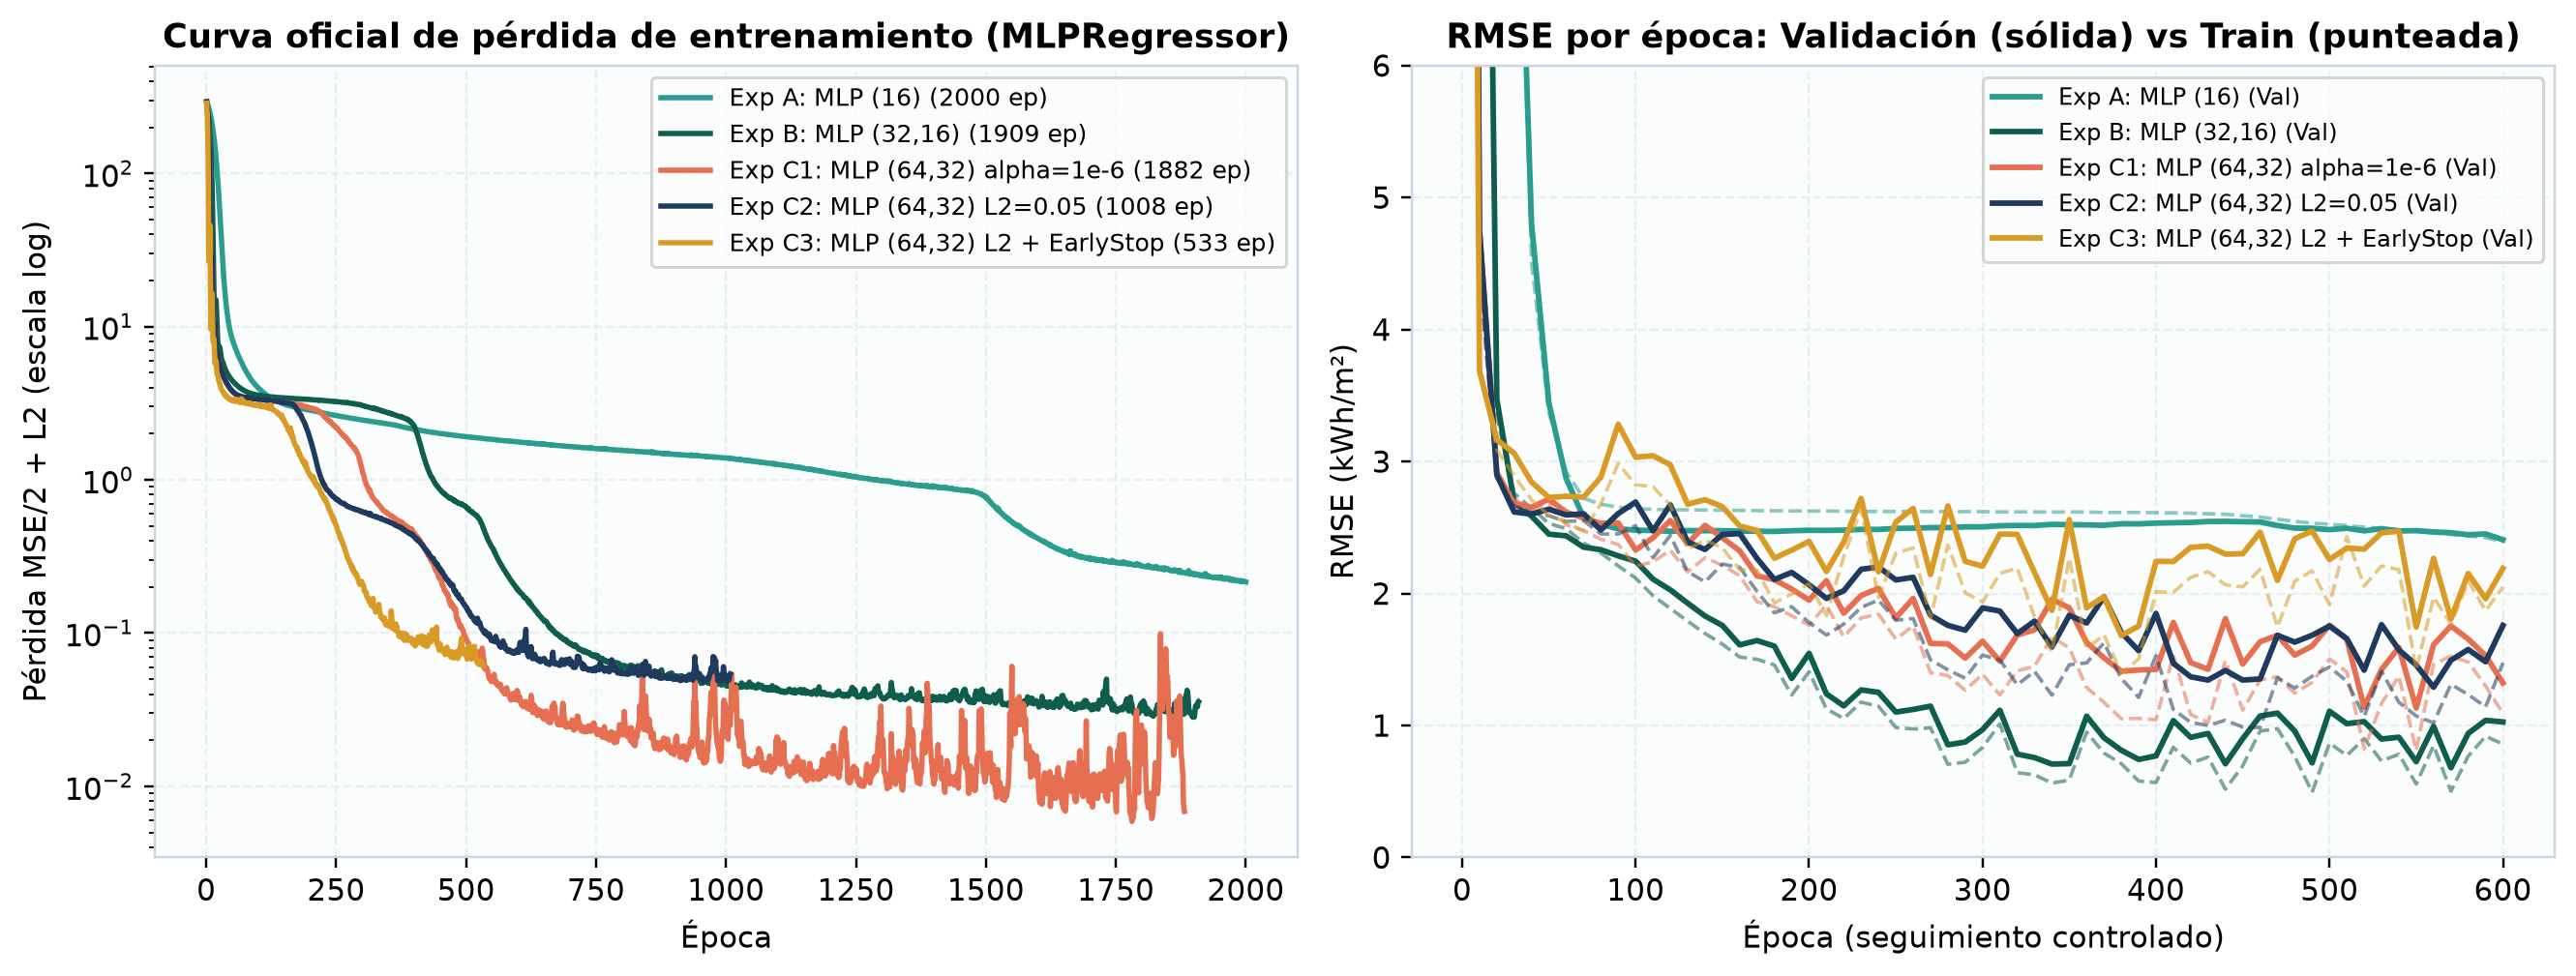
\includegraphics[width=0.98\textwidth]{../figures/fig04_curvas_perdida_mlp.png}
    \caption{Curvas de aprendizaje. Izquierda: pérdida oficial de \texttt{MLPRegressor} (nótese la meseta lineal inicial y la oscilación por sobreajuste de \texttt{C1} en naranja frente a la estabilidad de \texttt{B} y \texttt{C2}). Derecha: evolución de RMSE en Validación vs Train.}
    \label{fig:curvas}
\end{figure}

\begin{figure}[H]
    \centering
    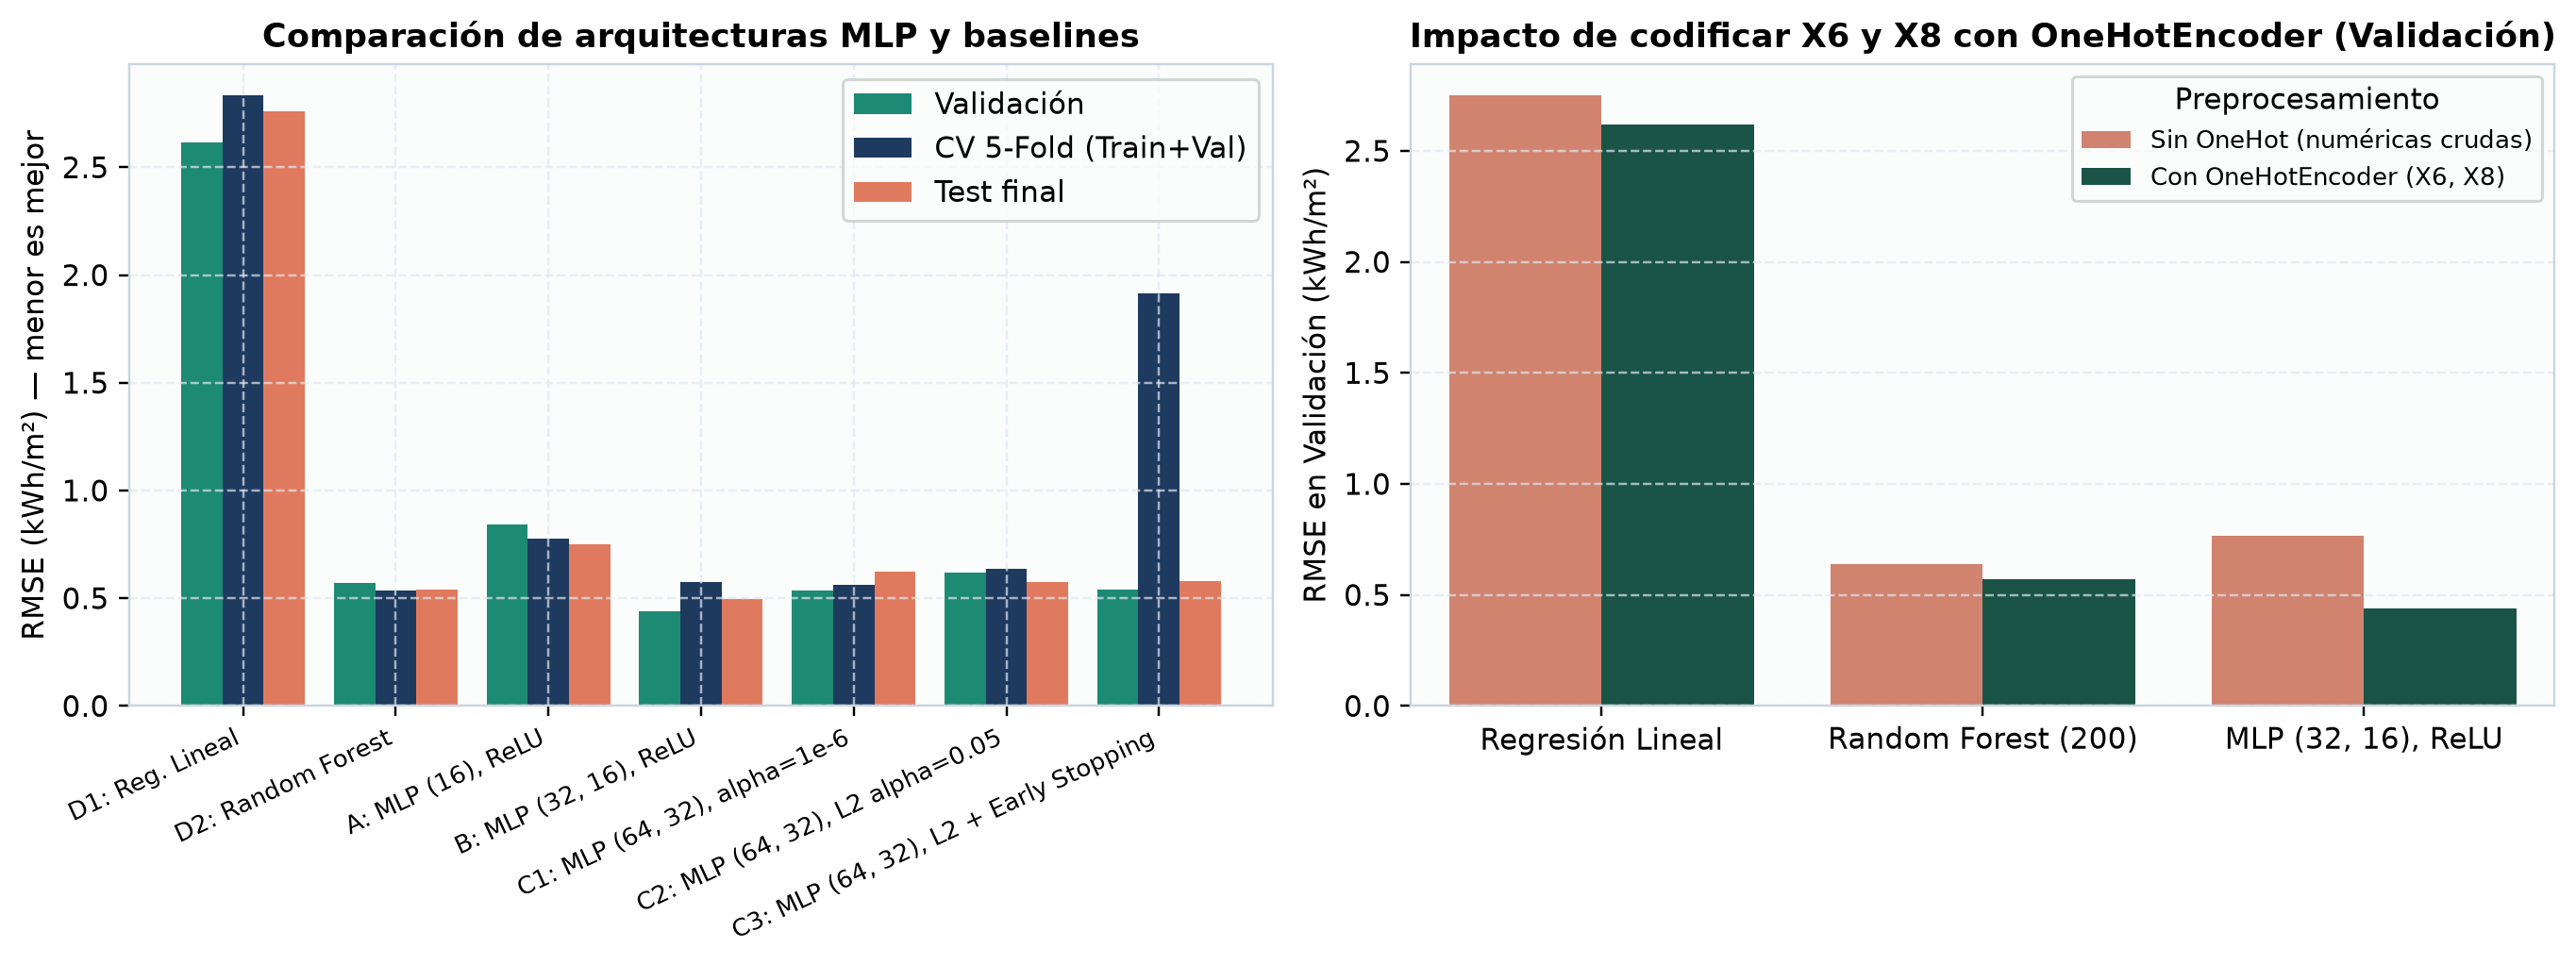
\includegraphics[width=0.98\textwidth]{../figures/fig05_comparacion_modelos.png}
    \caption{Comparación de RMSE en Validación, CV 5-Fold y Test (izquierda) y efecto de \texttt{OneHotEncoder} en $X_6, X_8$ (derecha).}
    \label{fig:comparacion}
\end{figure}

\begin{description}[leftmargin=0.8cm, style=nextline, itemsep=6pt]
    \item[Etapa 15 — Evaluación final, residuos y análisis por subgrupos (Test, $n=116$):]
    En el conjunto Test sellado, el ganador \textbf{MLP (32, 16)} logra $\text{MAE} = \mathbf{0.3757}$, $\text{RMSE} = \mathbf{0.4970\text{ kWh/m}^2}$ y $R^2 = \mathbf{0.9974}$, con una brecha mínima respecto a Validación ($\Delta\text{RMSE}_{\text{Test}-\text{Val}} = +0.0566\text{ kWh/m}^2$), confirmando excelente capacidad de generalización. En la Figura~\ref{fig:residuos}, los residuos de la Regresión Lineal muestran patrones curvos sistemáticos de hasta $\pm 7\text{ kWh/m}^2$, mientras que el MLP y Random Forest centran los errores cerca de cero.
\end{description}

\begin{figure}[H]
    \centering
    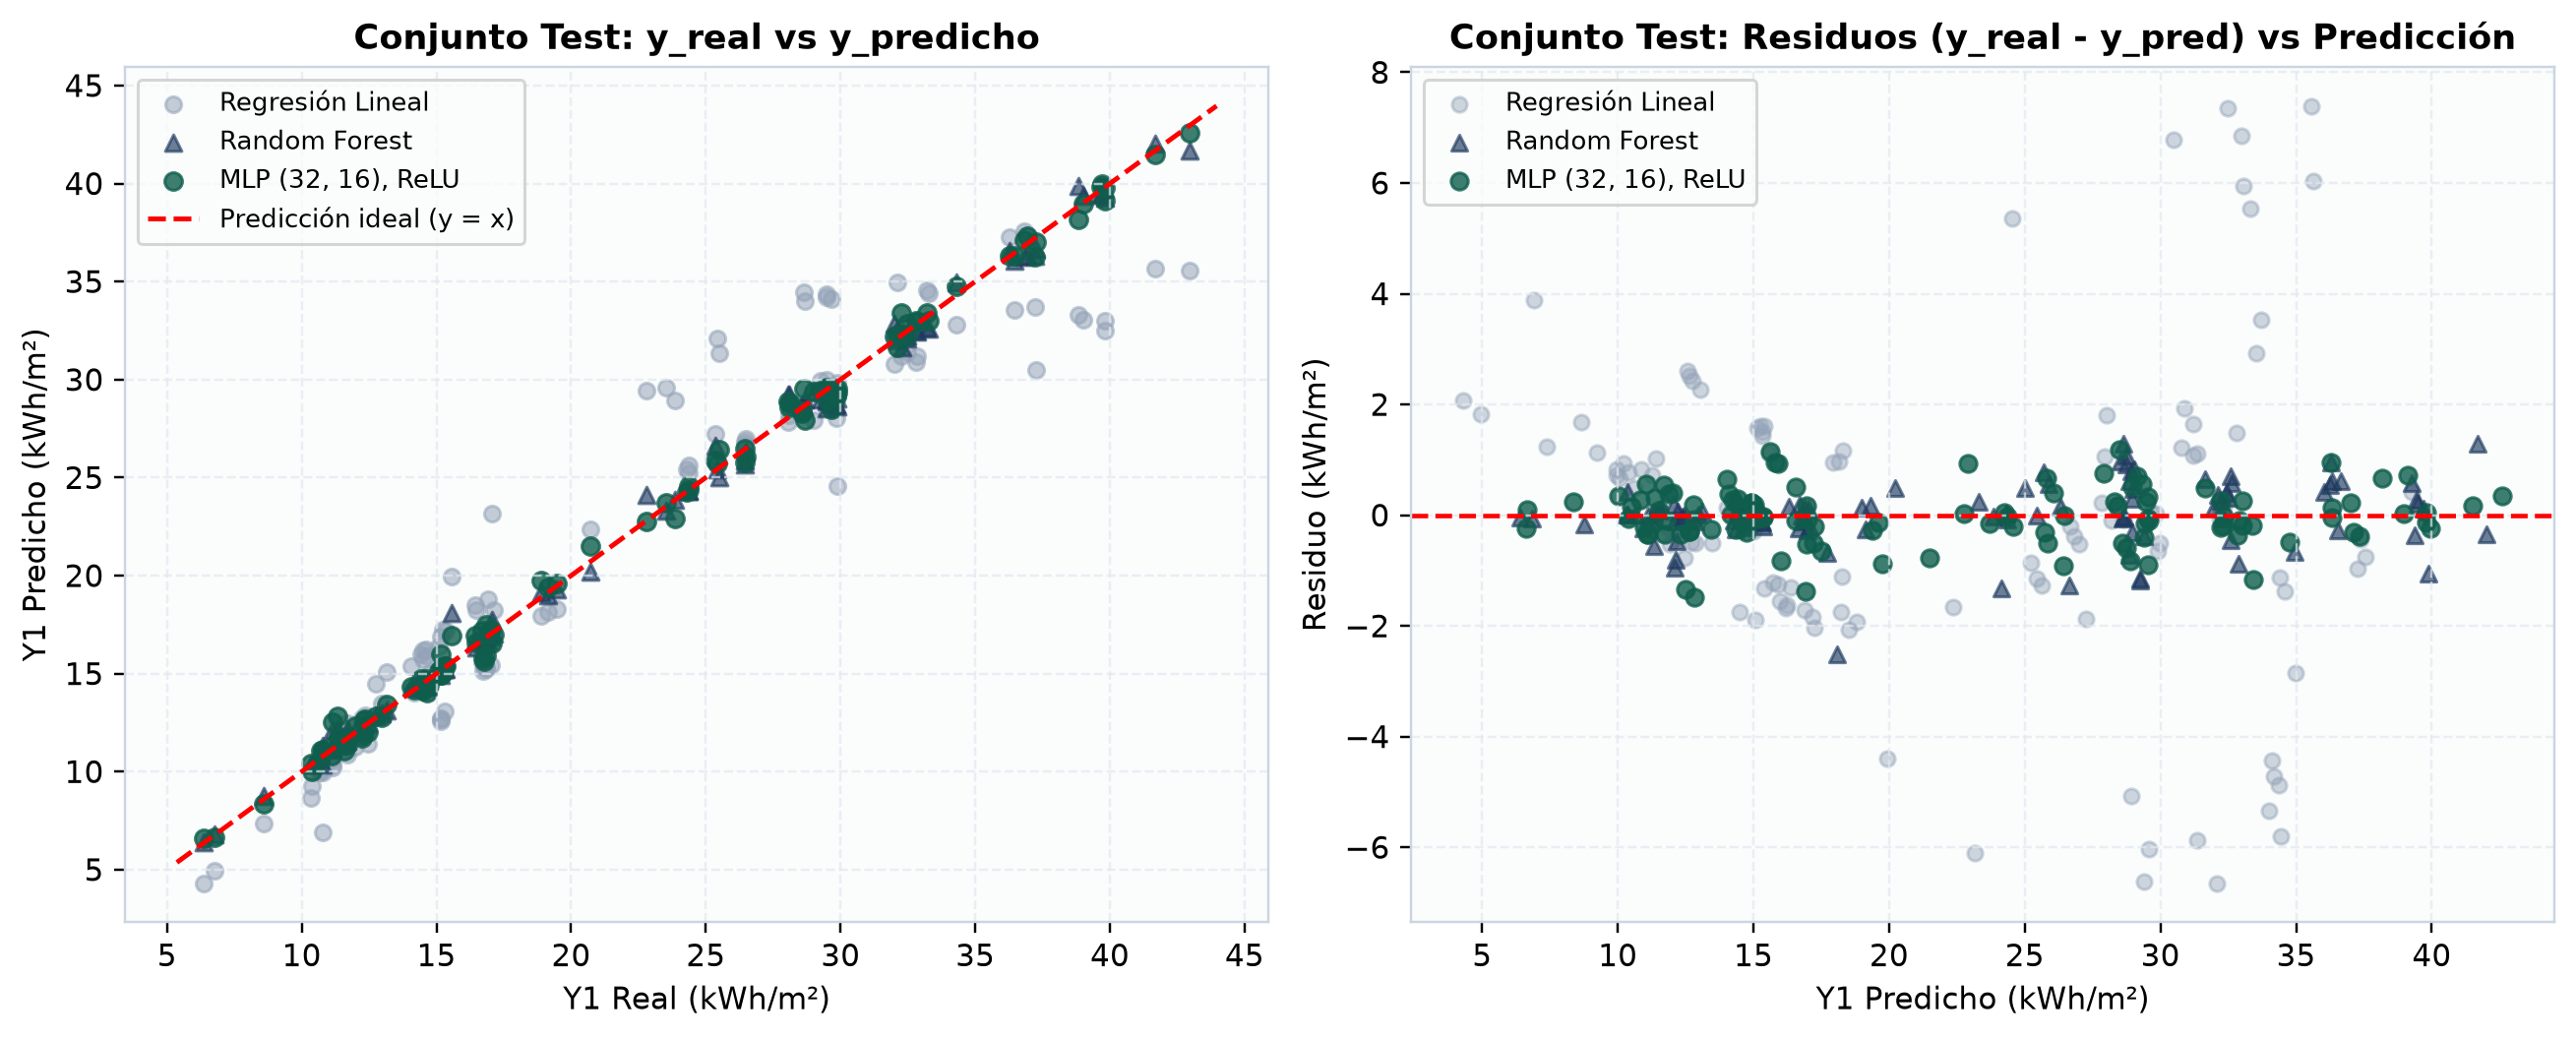
\includegraphics[width=0.98\textwidth]{../figures/fig06_real_vs_pred_y_residuos.png}
    \caption{Evaluación en Test ($n=116$): valores reales vs predichos (izquierda) y residuos $Y_{1,\text{real}} - Y_{1,\text{pred}}$ (derecha).}
    \label{fig:residuos}
\end{figure}

\begin{table}[H]
\centering
\caption{Evaluación en Test por subgrupos de Altura ($X_5$), Orientación ($X_6$) y Acristalamiento ($X_7$) para \texttt{MLP (32, 16)}.}
\label{tab:subgrupos}
\small
\begin{tabular}{llrrrrr}
\toprule
\textbf{Criterio} & \textbf{Subgrupo} & \textbf{$n_{\text{Test}}$} & \textbf{$Y_1$ medio} & \textbf{MAE} & \textbf{RMSE} & \textbf{$R^2$} \\
\midrule
\multirow{2}{*}{Altura ($X_5$)}
 & $3.5\text{ m}$ (1 planta) & 58 & 13.662 & 0.3482 & 0.4724 & 0.9717 \\
 & $7.0\text{ m}$ (2 plantas) & 58 & 30.712 & 0.4031 & 0.5204 & 0.9921 \\
\midrule
\multirow{4}{*}{Orientación ($X_6$)}
 & Norte (2) & 26 & 22.121 & 0.3405 & 0.4522 & 0.9975 \\
 & Este (3) & 32 & 26.374 & 0.4500 & 0.5457 & 0.9958 \\
 & Sur (4) & 32 & 18.520 & 0.3306 & 0.4567 & 0.9973 \\
 & Oeste (5) & 26 & 21.613 & 0.3749 & 0.5237 & 0.9976 \\
\midrule
\multirow{4}{*}{Acristalamiento ($X_7$)}
 & $0\%$ ($0.00$) & 8 & 14.465 & 0.5022 & 0.6354 & 0.9929 \\
 & $10\%$ ($0.10$) & 36 & 19.902 & 0.3709 & 0.5082 & 0.9963 \\
 & $25\%$ ($0.25$) & 36 & 23.427 & 0.3728 & 0.4734 & 0.9977 \\
 & $40\%$ ($0.40$) & 36 & 24.948 & 0.3553 & 0.4730 & 0.9976 \\
\bottomrule
\end{tabular}
\end{table}

\begin{figure}[H]
    \centering
    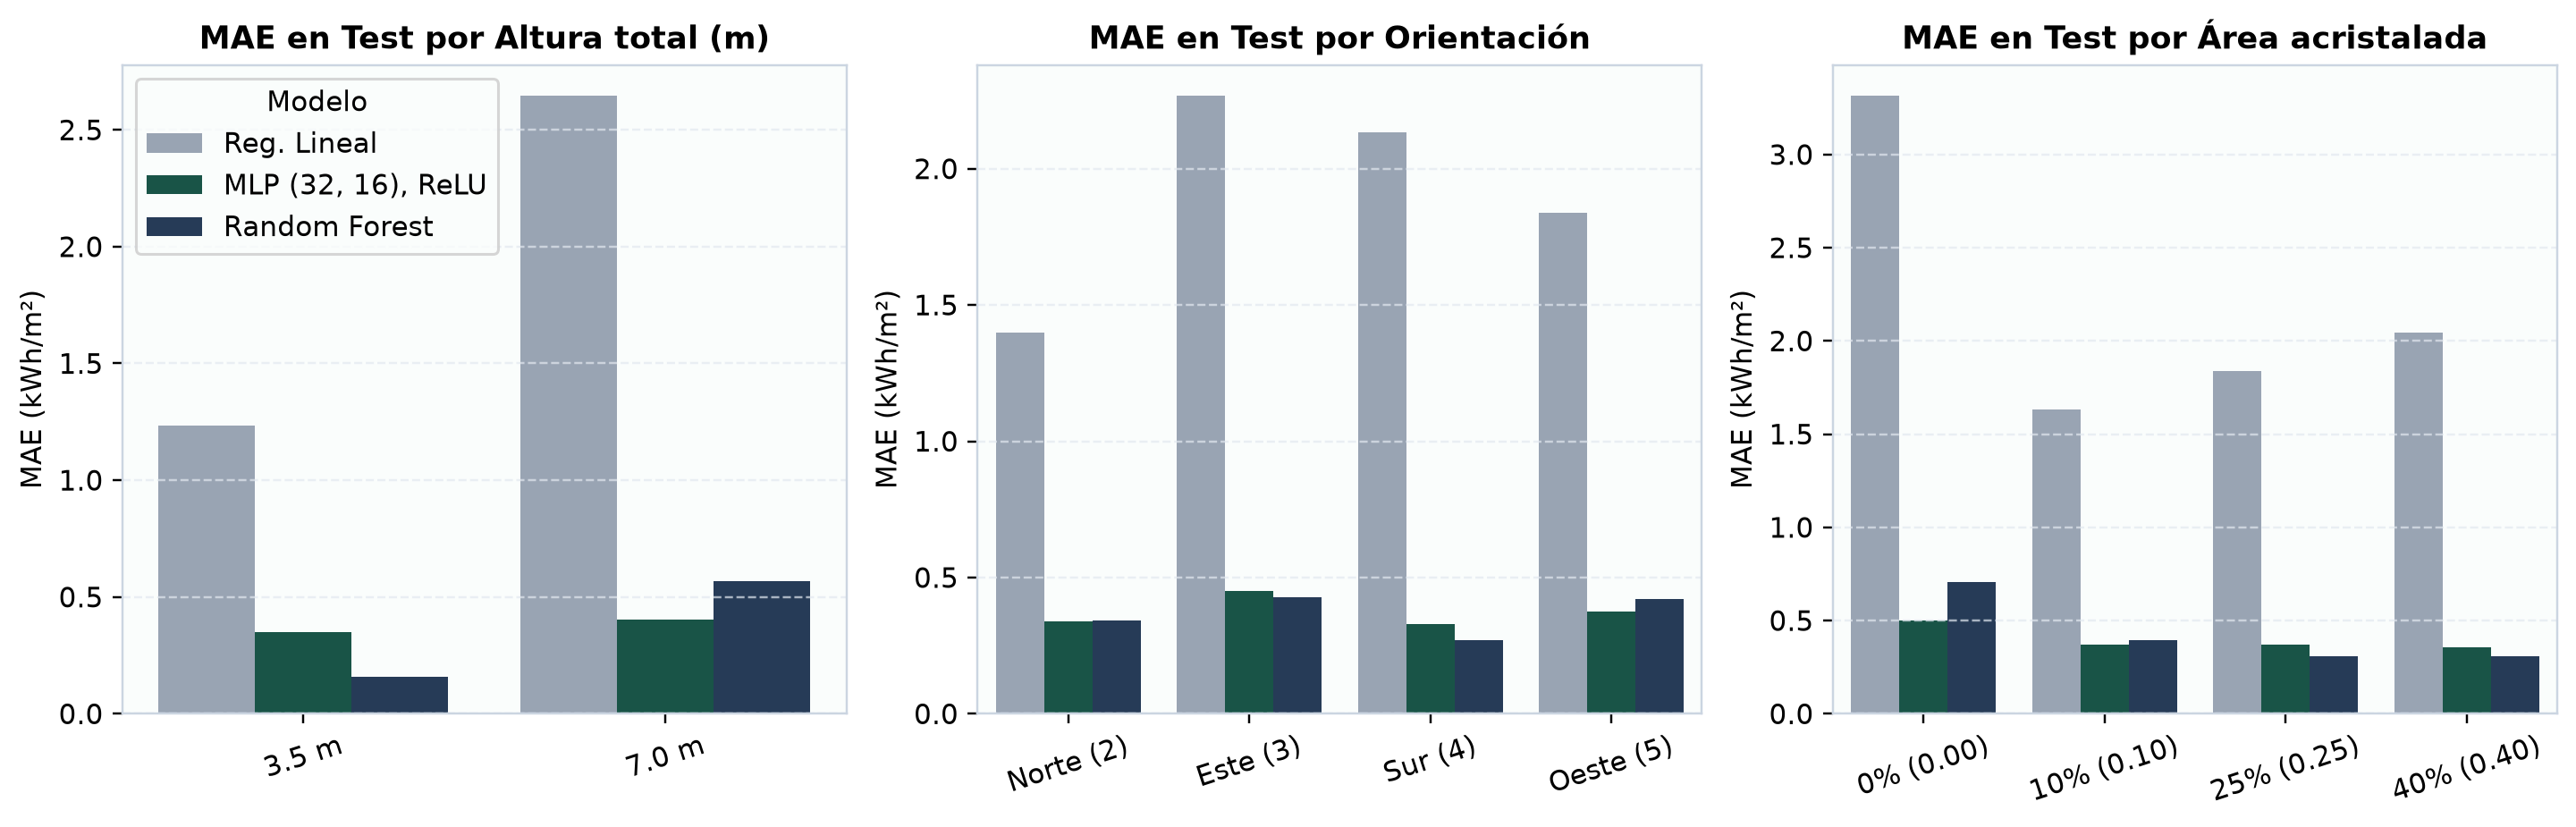
\includegraphics[width=0.98\textwidth]{../figures/fig07_errores_subgrupos.png}
    \caption{Comparación de MAE en Test por altura, orientación y porcentaje de acristalamiento. Destaca que en edificios de $7.0\text{ m}$ el MLP ($\text{MAE}=0.4031$) supera incluso a Random Forest ($\text{MAE}=0.5668$).}
    \label{fig:subgrupos}
\end{figure}

\begin{description}[leftmargin=0.8cm, style=nextline, itemsep=6pt]
    \item[Etapa 16 — Demostración Streamlit e interpretación de límites:]
    En \texttt{app.py} implementamos un simulador interactivo donde el usuario ingresa o elige perfiles de edificios y recibe la estimación en $\text{kWh/m}^2$ con banda orientativa ($\pm 1\text{ RMSE}$). Además, la función \texttt{check\_domain\_and\_geometry()} emite \textbf{alertas automáticas de extrapolación} si alguna variable sale de los rangos de entrenamiento (por ejemplo, altura distinta a $3.5\text{ m}$ ó $7.0\text{ m}$) o viola la identidad física del dataset ($X_2 \approx X_3 + 2 \cdot X_4$).
\end{description}

% ==============================================================================
% SECCIÓN 4: RESPUESTAS A LAS 8 PREGUNTAS DE SUSTENTACIÓN
% ==============================================================================
\section{Respuestas Claras a las 8 Preguntas de Sustentación}

\begin{enumerate}[leftmargin=1.4em,itemsep=7pt]
    \item \textbf{¿Por qué un MLP necesita funciones de activación no lineales?}\\
    Porque si no existiera una función no lineal como ReLU entre capas, multiplicar varias matrices seguidas ($W_3(W_2(W_1 x + b_1) + b_2) + b_3$) se colapsaría matemáticamente en una única recta ($W_{\text{eq}} x + b_{\text{eq}}$). Sin ReLU, nuestro MLP rendiría exactamente igual que la Regresión Lineal ($\text{RMSE} = 2.76$ en vez de $0.497$).

    \item \textbf{¿Qué aprende una capa oculta que no representa una regresión lineal simple?}\\
    Cada neurona oculta aprende combinaciones de diseño condicionadas por un umbral (``si la compacidad es baja \textit{y} la altura es 7 m, activa esta señal''). La segunda capa combina esas señales intermedias para formar superficies curvas suaves y capturar interacciones entre altura, forma y ventanas que una suma lineal única no puede modelar.

    \item \textbf{¿Por qué $X_6$ y $X_8$ requieren revisar su interpretación?}\\
    Aunque en el Excel vienen guardadas como números enteros ($X_6 \in \{2,3,4,5\}$, $X_8 \in \{0..5\}$), en realidad son \textbf{etiquetas nominales} (Norte, Este, Sur, Oeste; o tipo de reparto de ventanas). Tratarlas como números normales hace creer al modelo que ``Oeste (5) es más grande que Norte (2)''. Al convertirlas con \texttt{OneHotEncoder}, el RMSE del MLP en Validación bajó de $0.7653$ a $0.4397$ ($-42.5\%$).

    \item \textbf{¿Qué sucede si incluimos $Y_2$ como predictor de $Y_1$?}\\
    Ocurre \textbf{fuga de datos (\textit{data leakage})}. $Y_2$ (refrigeración) tiene una correlación de $0.9752$ con $Y_1$ (calefacción) porque ambas salen a la vez del mismo simulador térmico. Si la usamos como entrada, las métricas se inflan falsamente (Regresión Lineal baja a $\text{RMSE}=1.3793$), pero el modelo sería inútil en un proyecto real donde aún no se ha simulado ni medido $Y_2$.

    \item \textbf{¿Qué es \textit{early stopping} y cómo se utiliza sin tocar el test?}\\
    Es un freno automático que detiene el entrenamiento cuando el error sobre un subconjunto de vigilancia deja de mejorar por varias épocas seguidas (\texttt{n\_iter\_no\_change=60} en Exp.~C3), evitando que la red memorice ruido. Se aplica \textbf{sin tocar el Test} porque Scikit-learn aparta un 15\% (\texttt{validation\_fraction=0.15}) únicamente desde dentro del bloque de entrenamiento (\texttt{Train}), dejando el Test 100\% intacto.

    \item \textbf{¿Qué diferencias hay entre MAE y RMSE?}\\
    \textbf{MAE} (Error Absoluto Medio) promedia los errores tal cual están en $\text{kWh/m}^2$ ($\text{MAE}=0.3757$ significa que en promedio nos desviamos $\sim 0.38$ unidades). \textbf{RMSE} eleva cada error al cuadrado antes de promediar y saca raíz ($\text{RMSE}=0.4970$), por lo que \textbf{castiga mucho más los errores grandes o atípicos}. Cuando RMSE es bastante mayor que MAE, indica que hay casos puntuales con errores altos.

    \item \textbf{¿Por qué Random Forest podría superar al MLP en un conjunto pequeño?}\\
    Porque este dataset tiene solo 768 ejemplos (537 para entrenar) construidos sobre una rejilla discreta (12 formas exactas, 2 alturas exactas, 4 porcentajes de ventanas). Random Forest corta el espacio en cajas rectangulares que calzan naturalmente con diseños escalonados usando pocos datos ($\text{CV5 RMSE} = 0.5343$), mientras que un MLP necesita más datos y épocas para ajustar gradientes suaves sin sobreajustar.

    \item \textbf{¿Qué conclusiones respaldan los residuos?}\\
    En la gráfica de residuos ($Y_{1,\text{real}} - Y_{1,\text{pred}}$ vs predicción) de la Regresión Lineal se ven arcos pronunciados y errores de hasta $\pm 7\text{ kWh/m}^2$, demostrando \textbf{subajuste} por ignorar no linealidades. En cambio, en el \texttt{MLP (32, 16)} los residuos están centrados en cero (sesgo cercano a $0$) y casi todos dentro de $\pm 1.2\text{ kWh/m}^2$, observándose ligeramente mayor error en edificios sin ventanas ($0\%$, $n=8$ en Test, $\text{MAE}=0.5022$) por haber menos muestras de ese tipo.
\end{enumerate}

% ==============================================================================
% SECCIÓN 5: GUION COMPLETO DE 15 DIAPOSITIVAS PARA LA SUSTENTACIÓN (12 MIN)
% ==============================================================================
\section{Guion para Elaborar la Presentación (15 Diapositivas · 12 Minutos)}

La guía académica pide entre \textbf{12 y 18 diapositivas} cubriendo arquitectura, pipeline, resultados, errores y decisiones. A continuación se entrega el detalle listo para pasar al diseñador o armar las láminas.

\begin{table}[H]
\centering
\caption{Plan de tiempo sugerido (12 minutos de exposición + 5 minutos de preguntas).}
\small
\begin{tabular}{cllc}
\toprule
\textbf{Bloque} & \textbf{Diapositivas} & \textbf{Tema central} & \textbf{Tiempo} \\
\midrule
1 & Slides 1 -- 3 & Problema, datos UCI y exclusión de $Y_2$ & 2.0 min \\
2 & Slides 4 -- 6 & EDA, partición sin fuga y codificación $X_6, X_8$ & 2.5 min \\
3 & Slides 7 -- 9 & Teoría MLP en simple, diagrama original y experimentos A--D & 3.0 min \\
4 & Slides 10 -- 13 & Curvas, comparación final, residuos y subgrupos & 2.5 min \\
5 & Slides 14 -- 15 & Demo en Streamlit, limitaciones y conclusiones & 2.0 min \\
\bottomrule
\end{tabular}
\end{table}

\begin{enumerate}[leftmargin=1.4em, itemsep=6pt]
    \item \textbf{Slide 1 — Carátula:} Título del proyecto, Grupo 02, integrantes, asignatura y subtítulo ``Predicción de carga térmica de calefacción con MLP''.
    \item \textbf{Slide 2 — Problema y Propósito (Etapas 01–02):} Caso de la consultora energética. Poner visual de flujo: Plano ($X_1$--$X_8$) $\rightarrow$ MLP $\rightarrow$ $Y_1$ ($\text{kWh/m}^2$). Destacar origen simulado en \textit{Ecotect}.
    \item \textbf{Slide 3 — Dataset y Regla de $Y_2$ (Etapas 03–04):} Tabla compacta de las 8 entradas y caja roja de alerta sobre exclusión de $Y_2$ ($r = 0.9752$, evita \textit{data leakage}).
    \item \textbf{Slide 4 — Análisis Exploratorio (Etapa 05):} Insertar \texttt{fig01\_distribucion\_y1.png} y \texttt{fig02\_correlaciones.png}. Mensaje clave: $Y_1$ es bimodal por la altura ($3.5\text{ m}$ vs $7.0\text{ m}$).
    \item \textbf{Slide 5 — Relaciones clave del diseño (Etapa 05):} Insertar \texttt{fig03\_eda\_relaciones.png}. Explicar cómo compacidad, altura y área acristalada cambian el consumo.
    \item \textbf{Slide 6 — Separación y Preprocesamiento (Etapas 06–07):} Mostrar esquema 537 Train / 115 Val / 116 Test (\texttt{SEED=42}, Test sellado) + gráfico derecho de \texttt{fig05} (\texttt{OneHotEncoder} bajó el RMSE de $0.765$ a $0.440$).
    \item \textbf{Slide 7 — ¿Cómo funciona un MLP? (Fundamento teórico):} Explicar intuitivamente $z = Wx + b$, ReLU, salida lineal, MSE, retropropagación y Adam.
    \item \textbf{Slide 8 — Diagrama Original de la Arquitectura (Etapas 09–10):} Insertar el diagrama de la Figura~\ref{fig:arquitectura_mlp} ($16 \to 32 \to 16 \to 1 = 1{,}089$ parámetros). \textit{Requisito obligatorio de la guía.}
    \item \textbf{Slide 9 — Plan de Experimentos A--D (Etapas 08, 11, 13):} Tabla resumida comparando D0 Dummy, D1 Lineal, D2 Random Forest, A (16), B (32,16) y C1–C3 (64,32) con L2 y Early Stopping.
    \item \textbf{Slide 10 — Curvas de Pérdida y Sobreajuste (Etapa 12):} Insertar \texttt{fig04\_curvas\_perdida\_mlp.png}. Mostrar la meseta inicial, la oscilación de \texttt{C1} y el corte temprano de \texttt{C3} en 533 épocas.
    \item \textbf{Slide 11 — Selección y Comparación General (Etapas 13–14):} Insertar parte izquierda de \texttt{fig05\_comparacion\_modelos.png}. Justificar elección de \texttt{MLP (32,16)} por menor RMSE validado ($0.4404$) y simplicidad ($1{,}089$ params).
    \item \textbf{Slide 12 — Evaluación Final en Test y Residuos (Etapa 15):} Insertar \texttt{fig06\_real\_vs\_pred\_y\_residuos.png}. Destacar: Test RMSE = $0.4970$, $R^2 = 0.9974$ (vs Lineal $2.7612$ y RF $0.5406$).
    \item \textbf{Slide 13 — Análisis por Subgrupos (Etapa 15):} Insertar \texttt{fig07\_errores\_subgrupos.png}. Señalar que el MLP es el más preciso en edificios altos ($7.0\text{ m}$: $\text{MAE}=0.403$) y falla un poco más cuando $X_7=0\%$ ($n=8$).
    \item \textbf{Slide 14 — Demo en Vivo: Dashboard Streamlit (Etapa 16):} Mostrar capturas reales de \texttt{app.py} (Simulador con alertas de extrapolación fuera de rango e identidad geométrica $X_2 \approx X_3 + 2X_4$) y realizar prueba en vivo de 60 segundos.
    \item \textbf{Slide 15 — Limitaciones, Mejoras y Conclusiones:} Limitaciones (datos simulados, solo 2 alturas y clima fijo), mejora viable (incorporar datos climáticos reales o ajuste multi-objetivo conjunto con $Y_2$) y mensaje final de cierre.
\end{enumerate}

% ==============================================================================
% SECCIÓN 6: REFERENCIAS APA 7
% ==============================================================================
\section{Referencias (Formato APA 7)}

\begin{itemize}[leftmargin=1.5em, itemsep=6pt]
    \item Glorot, X., Bordes, A., \& Bengio, Y. (2011). Deep sparse rectifier neural networks. \textit{Proceedings of the Fourteenth International Conference on Artificial Intelligence and Statistics (AISTATS)}, \textit{15}, 315--323. \url{https://proceedings.mlr.press/v15/glorot11a.html}
    \item Goodfellow, I., Bengio, Y., \& Courville, A. (2016). \textit{Deep learning}. MIT Press. \url{https://www.deeplearningbook.org/}
    \item Kingma, D. P., \& Ba, J. (2015). Adam: A method for stochastic optimization. \textit{International Conference on Learning Representations (ICLR)}. \url{https://arxiv.org/abs/1412.6980}
    \item Pedregosa, F., Varoquaux, G., Gramfort, A., Michel, V., Thirion, B., Grisel, O., Blondel, M., Prettenhofer, P., Weiss, R., Dubourg, V., Vanderplas, J., Passos, A., Cournapeau, D., Brucher, M., Perrot, M., \& Duchesnay, É. (2011). Scikit-learn: Machine learning in Python. \textit{Journal of Machine Learning Research}, \textit{12}(85), 2825--2830. \url{https://scikit-learn.org/stable/modules/generated/sklearn.neural_network.MLPRegressor.html}
    \item Tsanas, A., \& Xifara, A. (2012). Accurate quantitative estimation of energy performance of residential buildings using statistical machine learning tools. \textit{Energy and Buildings}, \textit{49}, 560--567. \url{https://doi.org/10.1016/j.enbuild.2012.03.003}
    \item Tsanas, A., \& Xifara, A. (2012). \textit{Energy efficiency} [Conjunto de datos]. UCI Machine Learning Repository. \url{https://archive.ics.uci.edu/dataset/242/energy+efficiency}
\end{itemize}

\end{document}
